\documentclass[12pt]{article}
\usepackage{graphicx}
\usepackage{amssymb}
\usepackage{epstopdf}
\usepackage{amsmath}
\usepackage{multicol}
\usepackage{tcolorbox}
\usepackage{geometry}
\usepackage{enumitem}
\usepackage{fancyhdr}

\DeclareGraphicsRule{.tif}{png}{.png}{`convert #1 `dirname #1`/`basename #1 .tif`.png}

\textwidth = 6.5 in
\textheight = 9 in
\oddsidemargin = 0.0 in
\evensidemargin = 0.0 in
\topmargin = -23pt
\headheight = 0.0 in
\headsep = 0.0 in
\parskip = 0.2in
\parindent = 0.0in
\pagestyle{fancy}
\pagenumbering{gobble}

\newtheorem{theorem}{Theorem}
\newtheorem{corollary}[theorem]{Corollary}
\newtheorem{definition}{Definition}
%\includegraphics [height=50mm, width=50mm]{PathInt.jpg}
\title{Title} 

\begin{document}
%INSTRUCTOR NOTES

 Name:
 \begin{center}\large{3.4 Chain Rule}\end{center}

\begin{tcolorbox}

\textbf{Chain Rule:} \\
Let $z=g(x)$ and $y=f(z)$, so $y=f(g(x))$.\\

$$\frac{dy}{dx}=$$%=\frac{dy}{dz} \cdot \frac{dz}{dx}$$
\vspace{5mm}
$$\frac{d}{dx}f(g(x))=$$

\end{tcolorbox}

\begin{enumerate}
\item Consider the function $f\left(x\right)=\left(3x^{4}-5\right)^{3}-2.$ Rewrite $f\left(x\right)$ as a composition of functions, where $f\left(x\right)=v\left(u\left(x\right)\right).$ Find $v\left(x\right)$ and $u\left(x\right)$. Are these the only possibilities?
\vfill

\item Compute derivatives for the following functions. Assume $a$, $b$, and $c$ are constants:
\begin{multicols}{2}
\begin{enumerate}[itemsep=3cm]
\item $\displaystyle f(x)=\sqrt{3x^{2}-5x+3}$
\item $\displaystyle t(x)=(x^{3}+x)^{-1}$
\item $\displaystyle k(t)=e^{4t}$
\item $\displaystyle h(y)=\sqrt{e^{-\frac{y}{7}}+5}$
\item $\displaystyle g(t)=\left(1-e^{2\sqrt{t}}\right)^{19}$
\item $\displaystyle y(m)=\sqrt{e^{2m}+\sqrt{e^{3m}}}$
\item $\displaystyle f(w) = (bw^{a}+c)e^{w^{b}}$

\end{enumerate}
\end{multicols}



\newpage

\rhead{3.4 Chain Rule}
~
\item The function $f(x)$ is shown as the piecewise function with solid lines. The function $g(x)$ is the dotted line. Find the following:\\
\noindent\begin{minipage}{0.3\textwidth}% adapt widths of minipages to your needs
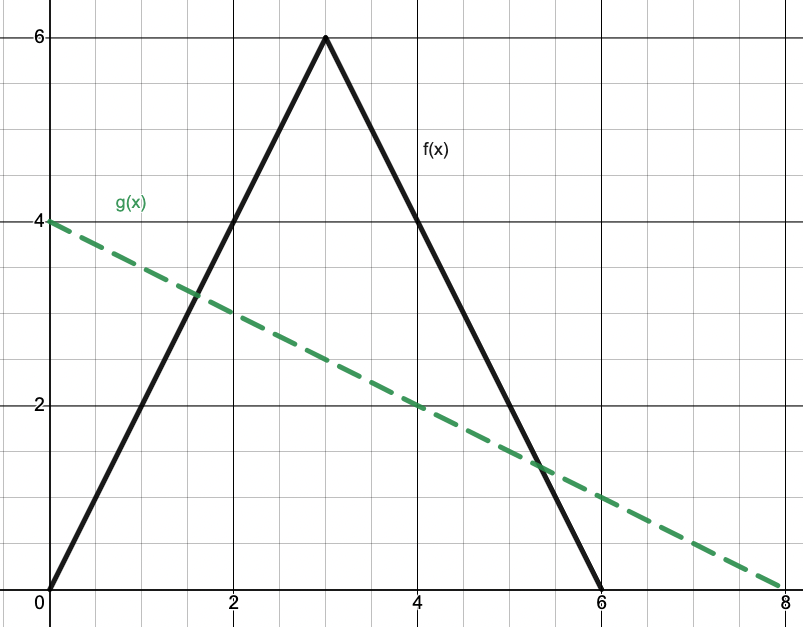
\includegraphics [height=50mm, width=50mm]{3_4_piece}
\end{minipage}%
\hspace{40mm}
\begin{minipage}{0.6\textwidth}
(a) $\displaystyle \frac{d}{dx}f\left(g\left(1\right)\right)$\\
\vspace{10mm}

(b) $\displaystyle \frac{d}{dx}e^{f\left(2\right)}$

\vspace{10mm}
\end{minipage}


\vfill


\item For $t$ in years since 2010, daily oil consumption in China, in thousands of barrels, was approximated by

$$B=8938e^{0.05t}.$$
	\begin{enumerate}
	\item Is daily oil consumption increasing or decreasing with time?
	\vfill
	\item How fast is oil consumption changing in 2020?
	\vfill
	\end{enumerate}
	\vfill

\end{enumerate}
\end{document} 

%%%%%%%%%



\item Consider the function $\displaystyle f(x)=e^{3x^2+5}$. Find functions $u(x)$ and $v(x)$ such that $f(x)$ can be rewritten as a composition $f(x)=u(v(x))$. Is this the only possibility?
\vfill
\item  Compute the following derivatives. 
	\begin{enumerate}
	\item $\displaystyle \frac{d}{dx} \left[ (2x^3+3)^2 \right]$
	\vfill
	\item $\displaystyle \frac{d}{dx}  \left[ e^{x^2}\right]$
	\vfill
	\item $\displaystyle \frac{d}{dx}  \left[ x(3x^4-2)\right]$
	\vfill
	\item $\displaystyle \frac{d}{dx} \left[  \frac{1}{x^2-e^x}\right]$
	\vfill
	\end{enumerate}
	
	
	
\begin{tcolorbox}
\textbf{Warm-up: } Solve the following equations for $t$.
\begin{multicols}{2}
\begin{enumerate}
\item $(t+1)^2=9$
\item $tx+x^2=5$
\end{enumerate}
\end{multicols}
\end{tcolorbox}

MINIPAGE
\noindent\begin{minipage}{0.3\textwidth}% adapt widths of minipages to your needs
try 1
\end{minipage}%
\hspace{40mm}
\begin{minipage}{0.6\textwidth}
a) $f'(2)=$\\\

b) $f'(4)=$\\

c) $f'(6)=$\\

d) $f'(7)=$\\

e) $f'(8)=$
\end{minipage}
